%% LyX 2.5.1 created this file.  For more info, see https://www.lyx.org/.
%% Do not edit unless you really know what you are doing.
\documentclass[brazil]{article}
\usepackage[T1]{fontenc}
\usepackage[utf8]{luainputenc}
\usepackage{colortbl}
\usepackage{amsmath}
\usepackage{graphicx}
\usepackage{geometry}
\geometry{verbose,tmargin=3cm,bmargin=3cm,lmargin=3cm,rmargin=2.5cm}

\makeatletter

%%%%%%%%%%%%%%%%%%%%%%%%%%%%%% LyX specific LaTeX commands.
%% Because html converters don't know tabularnewline
\providecommand{\tabularnewline}{\\}

%%%%%%%%%%%%%%%%%%%%%%%%%%%%%% User specified LaTeX commands.
\usepackage{babel}








\makeatother

\usepackage{babel}
\begin{document}
\title{Aprendizado de Máquina }
\maketitle

\subsection{Modelo McCulloch-Pitts}

Para que seja possível iniciar uma discussão acerca de redes neurais artificiais, é necessário voltar a atenção para o primeiro modelo de neurônio biológico proposto por McCulloch e Pitts em 1943. Este é o modelo mais clássico de neurônio em RNA (redes neurais artificiais), proposto em um trabalho intitulado ``Um cálculo lógico das ideias intrínsecas da atividade neural'' \cite{zuben_attux}.

Em um neurônio biológico, as sinapses possuem canais que permitem a entrada e saída de íons de modo que torna o neurônio capaz de receber sinais de entrada através da mesma. Dependendo da intensidade resultante destes sinais de entrada, isto é, se a intensidade resultante for superior a um determinado limiar, o neurônio libera neurotransmissores na sinapse, o que por sua vez corresponde à emissão de um sinal de saída.

McCulloch e Pitts então empreenderam a primeira tentativa de entender a atividade neural a partir de unidades elementares da computação, construindo um modelo baseado em simplificações do que se sabia na época sobre o neurônio biológico. Seu modelo é baseado principalmente nas seguintes premissas \cite{zuben_attux},\cite{jacson}: 
\begin{itemize}
\item O neurônio tem apenas dois estados: ativo ($1$) ou inativo ($0$); 
\item Uma certa quantidade fixa de sinapses deve ser excitada de forma a excitar o neurônio; 
\item A atividade de uma sinapse inibitória bloqueia completamente a atividade do neurônio. 
\end{itemize}
Matematicamente então, o neurônio de McCulloch Pitts, a cada iteração: 
\begin{itemize}
\item Soma as entradas com peso unitário $\sum_{j}x_{j}$; 
\item Se esse valor ultrapassar um limiar $\theta$, e a entrada inibitória $x_{i}$ não estiver ativa ($0$), o neurônio é ativado ($1$); 
\item Se não, o neurônio permanece inativo ($0$). 
\end{itemize}
Isto é: 
\begin{equation}
f\left(x_{1},\dots,x_{N}\right)=\left\{ \begin{array}{ccccc}
1 & se & \sum^{N}_{j=1}x_{j}>\theta & e & x_{i}=0\\
0 & se & \sum^{N}_{j=1}x_{j}\leq\theta & ou & x_{i}=1
\end{array}\right..
\end{equation}

Evidentemente, esse modelo apresenta algumas limitações, dentre elas pode-se destacar que o mesmo não é capaz de aprender a partir dos dados disponíveis nem diferenciar a importância das entradas e, por fim, a entrada inibitória ainda pode ser uma limitação inconveniente.

\subsection{Modelo de Rosenblatt}

Nos anos de 1950 e 1960, Frank Rosenblatt, inspirado pelo trabalho de Warren McCulloch e Waltper Pitts, desenvolve seu próprio modelo, conhecido também como perceptron \cite{nielsen2015neural}. Rossenblatt propôs modificações simples para o cálculo da saída, dentre as quais pode-se destacar a introdução de pesos diferentes para cada entrada e a remoção da entrada inibitória.

Utilizando os pesos, foi capaz de expressar as diferentes importâncias que cada entrada poderia possuir. Então sendo o peso $w_{j}$ correspondente à entrada $x_{j}$ e mantendo a notação do limiar $\theta$, a saída do neurônio $f$ é dada por: 
\begin{equation}
f\left(x_{1},\dots,x_{N}\right)=\left\{ \begin{array}{ccc}
1 & se & \sum^{N}_{j=1}w_{j}x_{j}>\theta\\
0 & se & \sum^{N}_{j=1}w_{j}x_{j}\leq\theta
\end{array}\right..
\end{equation}
Onde foi pequena alteração da notação, o limiar foi passado para outro lado da igualdade, onde recebe o nome de viés ($b=-\theta$) . Isto é: 
\begin{equation}
f\left(x_{1},\dots,x_{N}\right)=\left\{ \begin{array}{ccc}
1 & se & \sum^{N}_{j=1}w_{j}x_{j}+b>0\\
0 & se & \sum^{N}_{j=1}w_{j}x_{j}+b\leq0
\end{array}\right.\rightarrow f\left(x_{1},\dots,x_{N}\right)=\left\{ \begin{array}{ccc}
1 & se & \sum^{N}_{j=1}w_{j}x_{j}>\theta\\
0 & se & \sum^{N}_{j=1}w_{j}x_{j}\leq\theta
\end{array}\right.
\end{equation}
o somatório do produto entre pesos e entradas pode ser escrito como um produto interno, utilizando a notação da Mecânica Quântica: 
\begin{equation}
f=\left\{ \begin{array}{ccc}
1 & se & \left\langle w|x\right\rangle +b>0\\
0 & se & \left\langle w|x\right\rangle +b\geq0
\end{array}\right..
\end{equation}
Onde: 
\begin{equation}
\left\langle w|x\right\rangle =\overrightarrow{w}\cdot\overrightarrow{x}=\left[\begin{array}{cccc}
w_{1} & w_{2} & \cdots & w_{N}\end{array}\right]^{T}\left[\begin{array}{c}
x_{1}\\
x_{2}\\
\vdots\\
x_{N}
\end{array}\right]=\sum^{N}_{j=1}w_{j}x_{j}.
\end{equation}
Pode-se perceber que o viés é equivalente a uma entrada $x_{b}=b$ com um peso $w_{b}=1$. Um exemplo prático da usabilidade de perceptrons é a possibilidade de construção da porta lógica NAND. Considerando um perceptron com um viés de $b=3$ e duas entradas com pesos iguais $w_{1}=w_{2}=-2$, e passando a denotar o somatório como função ativação $z\left(x_{1},x_{2}\right)$ tem-se: 
\begin{equation}
z=-2x_{1}-2x_{2}+3.
\end{equation}
A partir da função ativação é possível construir a seguinte tabela de entradas e saídas: 
\begin{center}
\begin{tabular}{|l|l|l|l|}
\hline 
$x_{1}$  & $x_{2}$  & $z$  & $f$ \tabularnewline
\hline 
0  & 0  & 3  & 1 \tabularnewline
\hline 
1  & 0  & 1  & 1 \tabularnewline
\hline 
0  & 1  & 1  & 1 \tabularnewline
\hline 
1  & 1  & -1  & 0 \tabularnewline
\hline 
\end{tabular}
\par\end{center}

Esta tabela é idêntica a tabela verdade da porta NAND. A NAND é uma porta universal para a computação clássica. Deste modo, o perceptron também é universal para a computação clássica, e através de uma rede de perceptrons é possível computar qualquer função lógica \cite{nielsen2015neural}.

Porém, a maior novidade que surge em comparação ao modelo anterior, é que uma vez que a entrada inibitória pode ser simulada por entradas simples \cite{rojas}, a remoção dela junto com as outras modificações propostas por Rosenblatt tornou seu modelo mais flexível, e concedeu a capacidade ao perceptron de ter seus pesos e viés atualizados através de um algoritmo de aprendizado. Isto é, sem uma intervenção direta pelo programador. O algoritmo de aprendizagem nos permite resolver problemas que são extremamente difíceis de se propor um modelo diretamente, um exemplo que podemos citar são problemas de classificação de imagens.

\subsubsection{Regra de aprendizado}

Rosenblatt provou que a regra de aprendizado proposta em seu trabalho sempre converge para os pesos corretos para resolver o problema em questão, se estes pesos existirem. A regra de aprendizado também é conhecida como algoritmo de aprendizado, ou algoritmo de treinamento \cite{NND}. O algoritmo do perceptron é do tipo aprendizado supervisionado. Isto significa que é fornecido um conjunto de exemplos (dados de treinamento) do comportamento apropriado da rede: 
\begin{equation}
\left\{ \left|x_{1}\right\rangle ,t_{1}\right\} ,\left\{ \left|x_{2}\right\rangle ,t_{2}\right\} ,\dots,\left\{ \left|x_{N}\right\rangle ,t_{N}\right\} .
\end{equation}
Onde $t_{j}$ é o saída desejada correspondente à entrada $\left|x_{j}\right\rangle $. Então a regra de aprendizado é usada para ajustar os pesos e o viés do neurônio de modo a mover as saídas do mesmo para mais próximo às saídas desejadas. Um conceito importante é a fronteira de decisão. Esta é definida para quando a função de ativação é igual a zero, isto é: 
\begin{equation}
z=\left\langle w|x\right\rangle +b=0.
\end{equation}
A fronteira de decisão é um hiperplano (um sub-espaço de dimensão $N-1$ em um espaço de dimensão $N$) no espaço de entrada. Para ficar mais concreto, como exemplo pode-se restringir a análise à duas entradas, então se o espaço de entrada tem 2 dimensões $\left(x_{1},x_{2}\right)=\left(x,y\right)$, logo o hiperplano é uma reta (1 dimensão) em que a saída é $0$ de um lado e $1$ do outro. Especificamente: 
\begin{equation}
\begin{split}x_{1}w_{1}+w_{2}x_{2}+b=0,\\
x_{2}=-\frac{w_{1}}{w_{2}}x_{1}-\frac{b}{w_{2}}.
\end{split}
\end{equation}
Isto é uma equação da reta do tipo $y=ax+b$ onde $a=-\frac{w_{1}}{w_{2}}$ e $b=-\frac{b}{w_{2}}$. Sendo $a$ a inclinação da reta, um vetor perpendicular a fronteira de decisão deve ter a inclinação $\left(-\frac{1}{a}\right)=\frac{w_{2}}{w_{1}}$. Portanto o vetor peso $\left|w\right\rangle $ é perpendicular a reta formada pela fronteira de decisão. Desta maneira, este perceptron é capaz de classificar corretamente um conjunto de dados de duas dimensões no qual as duas classes podem ser separadas por uma reta. O algoritmo de aprendizado é responsável por ajustar a inclinação (através dos pesos) e a distância da origem (pelo viés) desta reta.

Desta maneira, é possível compreender as regras de aprendizado do perceptron para atualização dos pesos em 3 regras: 
\begin{itemize}
\item Se foi classificado corretamente, não realizamos nenhuma alteração; 
\item Se era para ser classificado como $t=1$, e foi classificado errado $f=0$, soma-se o vetor de entrada: $\left|w\right\rangle '=\left|w\right\rangle '+\left|x\right\rangle $; 
\item Se era para ser classificado como $t=0$, e foi classificado errado $f=1$, subtrai o vetor de entrada: $\left|w\right\rangle '=\left|w\right\rangle '-\left|x\right\rangle $. 
\end{itemize}
Dessa maneira, aproxima-se o vetor peso $\left|w\right\rangle $ do vetor de entrada $\left|x\right\rangle $ quando a classificação deveria ser $t=1$ e o foi classificado errado, e afasta-se quando a classificação correta é $t=0$ mas foi classificado incorretamente. Essas três regras ainda podem ser unificadas ao se notar que o sinal da operação com o vetor $\left|x\right\rangle $ pode ser descrito pela diferença $e=\left(t-f\right)$, que nada mais é do que uma medida simples do erro. Dessa maneira, de forma unificada pode-se escrever: 
\begin{equation}
\left|w\right\rangle '=\left|w\right\rangle '+e\left|x\right\rangle .
\end{equation}
E lembrando que o viés pode ser descrito como um peso para uma entrada em que a entrada é $x_{j}=1$, de maneira análoga: 
\begin{equation}
b'=b+e.
\end{equation}
A fim de aumentar o controle sobre a aprendizagem, pode-se considerar ainda uma taxa de aprendizado $\eta$ : 
\begin{equation}
\begin{split}\left|w\right\rangle ' & =\left|w\right\rangle '+e\eta\left|x\right\rangle ,\\
b' & =b+\eta e.
\end{split}
\end{equation}
Perceptrons ainda são naturalmente limitados, essas limitações foram demonstradas em um livro chamado Perceptrons por Marvin Minsky e Seymour Papert. A fronteira de decisão do perceptron é linear, logo um perceptron pode ser usado para classificar problemas que podem ser descritos de maneira linearmente separável, porém infelizmente muitos problemas não são linearmente separáveis, como a porta lógica XOR \cite{NND}.

\subsection{Modelo Sigmoide}

Outra limitação mais evidente do modelo do perceptron se encontra nos valores de saída que são binários. Além disso a regra de aprendizado foi desenhada para atualizar os valores de cada perceptron individualmente, então para a construção de uma rede neural em que se utiliza a saída de um perceptron ($p_{11}$) como entrada de outro perceptron ($p_{12}$), seria necessário saber qual é o valor intermediário esperado (a saída de $p_{11}$, que serve de entrada para $p_{12}$). Deste modo, para a construção de uma rede neural mais complexa, é necessário também um modelo genérico mais complexo.

Sigmoide é um tipo de neurônio artificial similar aos perceptrons, porém modificado para que pequenas variações nos pesos e viés causem apenas uma pequena variação na saída, uma vez que agora a saída é um valor contínuo. É por isso que sigmoides são os principais modelos de neurônios e junto com o algoritmo de aprendizado do gradiente descendente permitem a construção de redes mais complexas.

Para atingir esse objetivo, o neurônio sigmoide aceita entradas e saída entre $0$ e $1$, ou seja, não trabalha mais apenas com valores binários na saída. A função ativação clássica de um sigmoide é: 
\begin{equation}
f\left(x_{1},\dots,x_{N}\right)\equiv\frac{1}{1+e^{-\left(\left\langle w|x\right\rangle -b\right)}}.
\end{equation}
Pode-se conferir que para casos extremos em que $g=\left\langle w|x\right\rangle -b\rightarrow\infty$ e $g=\left\langle w|x\right\rangle -b\rightarrow-\infty,$ a função vale respectivamente: 
\begin{equation}
\begin{split}\lim_{g\rightarrow\infty}f & =\lim_{g\rightarrow\infty}\frac{1}{1+e^{-g}}=1,\\
\lim_{g\rightarrow-\infty}f & =\lim_{g\rightarrow-\infty}\frac{1}{1+e^{-g}}=0.
\end{split}
\end{equation}
Desta maneira, a função sigmoide mantém a saída entre os valores $0$ e $1$, porém não mais de forma binária, mas de maneira suave.

\subsubsection{Gradiente descendente}

A mudança na função de ativação do neurônio sigmoide permite que seja utilizado um novo algoritmo de aprendizado, mais complexo, mas que também permite a construção de redes mais complexas. Como a regra de aprendizado visa aproximar os pesos e viés de maneira que o resultado da rede se aproxime do resultado esperado, é interessante que seja possível quantificar o erro da rede ao classificar um conjunto de dados de treinamento. Assim, pode-se concentrar em minimizar esse valor.

Com esta finalidade define-se uma função custo, isto é, uma função que serve exatamente para quantificar o erro. Considerando que a rede pode apresentar mais de uma saída, pode-se escrever o vetor de saídas desejadas para um determinado vetor de entrada $\left|x_{j}\right\rangle $ como $\left|d_{j}\right\rangle $ . De forma mais explícita, para $M$ saídas possíveis temos $\left|d_{j}\right\rangle =\left[\begin{array}{cccc}
d_{j1} & d_{j2} & \dots & d_{jM}\end{array}\right]^{T}$. Então o elemento $d_{ji}$ corresponde à saída desejada pelo neurônio $i$ para o vetor de entrada $j$. De forma análoga, pode-se escrever o vetor dos resultados obtidos pela rede como $\left|f_{j}\right\rangle $. A partir desta notação, uma típica função custo pode ser escrita, para $N$ pesos e $K$ entradas, como \cite{nielsen2015neural}: 
\begin{equation}
C\left(w_{1},\dots,w_{N},b\right)=\frac{1}{2K}\sum^{K}_{j=1}\left\Vert \left|d_{j}\right\rangle -\left|f_{j}\right\rangle \right\Vert ^{2}.
\end{equation}
Onde a norma de um vetor $\left|x\right\rangle $ é definida como $\left\Vert \left|x\right\rangle \right\Vert =\sqrt{\left\langle x|x\right\rangle }$. Quando os pesos são atualizados, a expectativa é de que ocorra uma diminuição do valor da função custo, isto é, uma variação negativa. Para tornar os cálculos mais compactos, uma alternativa é absorver o viés no vetor dos pesos como um peso $w_{N+1}=b$. 
\begin{equation}
\left|w\right\rangle =\left[\begin{array}{c}
w_{1}\\
w_{2}\\
\vdots\\
w_{N}\\
b
\end{array}\right]=\left[\begin{array}{c}
w_{1}\\
w_{2}\\
\vdots\\
w_{N}\\
w_{N+1}
\end{array}\right]\qquad\left|x\right\rangle =\left[\begin{array}{c}
x_{1}\\
x_{2}\\
\vdots\\
x_{N}\\
1
\end{array}\right]=\left[\begin{array}{c}
x_{1}\\
x_{2}\\
\vdots\\
x_{N}\\
x_{N+1}
\end{array}\right].
\end{equation}
A diferencial total da função custo é dada por: 
\begin{equation}
\begin{split}dC & =\sum^{N+1}_{j=1}\frac{\partial C}{\partial w_{j}}dw_{j},\\
\Delta C & \approx\sum^{N+1}_{j=1}\frac{\partial C}{\partial w_{j}}\Delta w_{j}.
\end{split}
\end{equation}
Pela definição do gradiente para $N+1$ dimensões do espaço de pesos temos $\nabla_{w}\equiv\sum^{N+1}_{j=1}\widehat{w}_{j}\frac{\partial}{\partial w_{j}}$, e definindo um vetor de variações dos pesos como $\left|\Delta w\right\rangle =\sum^{N+1}_{j=1}\Delta w_{j}\widehat{w}_{j}$, é possível então reescrever a variação da função custo como: 
\begin{equation}
\Delta C\approx\nabla_{w}C\cdot\left|\Delta w\right\rangle .
\end{equation}
Supondo uma variação no vetor peso da seguinte forma: $\left|\Delta w\right\rangle =-\eta\nabla_{w}C$, espera-se que a função custo seja minimizada. Pois a diferencial da função custo torna-se, desde que a variação proposta seja pequena o suficiente: 
\begin{equation}
\begin{split}\Delta C & \approx\nabla_{w}C\cdot\left|\Delta w\right\rangle ,\\
 & \approx\nabla_{w}C\cdot\left(-\eta\nabla_{w}C\right),\\
 & \approx-\eta\left\Vert \nabla_{w}C\right\Vert ^{2}.
\end{split}
\end{equation}
Onde $\eta$ é chamada de taxa de aprendizado, análogo ao caso do perceptron. Portanto o algoritmo do gradiente descendente consiste em atualizar os pesos da seguinte forma: 
\begin{equation}
\begin{split}\left|w\right\rangle ' & =\left|w\right\rangle +\left|\Delta w\right\rangle ,\\
 & =\left|w\right\rangle -\eta\nabla_{w}C.
\end{split}
\end{equation}
E o gradiente da função custo, de forma mais específica: 
\begin{equation}
\begin{split}\nabla_{w}C & =\frac{1}{2K}\sum^{N}_{j=1}\left(\nabla_{w}\left\Vert \left|d_{j}\right\rangle -\left|f_{j}\right\rangle \right\Vert ^{2}\right)\\
 & =\frac{1}{K}\sum^{K}_{j=1}\left(\left\Vert \left|d_{j}\right\rangle -\left|f_{j}\right\rangle \right\Vert \right)\left(\nabla_{w}\left\Vert \left|d_{j}\right\rangle -\left|f_{j}\right\rangle \right\Vert \right).
\end{split}
\end{equation}
Isto decorre da regra da cadeia. Vale destacar que enquanto $\left|d_{j}\right\rangle $ é um vetor de constantes, o vetor $\left|f_{j}\right\rangle $ é formado por elementos $f_{ji}$ que são obtidos através da função de ativação. O primeiro termo entre parênteses no gradiente da função custo é simplesmente a diferença entre os resultados desejados e o obtido pela rede. Como a regra de aprendizado é aplicada depois da rede classificar os dados de treinamento, isto pode ser obtido diretamente a partir dos valores resultantes, sendo assim, resta unicamente a tarefa de calcular o segundo termo, que vai depender de detalhes específicos da rede.

Apesar de envolver um cálculo mais complicado que para o caso do perceptron, este algoritmo de aprendizado possui a vantagem de que só é necessário saber as saídas desejadas de toda a rede para aplicar a regra de aprendizado em cada um dos neurônios que compõem esta mesma rede.

\subsection{Método Kernel}

Perceptrons e sigmoides são modelos que são relativamente fáceis de implementar e otimizar, mas são classificadores lineares, isto é, são limitados a fronteiras de decisões lineares, é para lidar com essa questão que surge o método kernel. Este método tem como principal objetivo capturar padrões não-lineares nos dados mapeando-os em dimensões mais elevadas no qual exibem um padrão linear \cite{kernel2}. Isto é feito à custas de um aumento no custo computacional necessário para realizar o treinamento. Porém, uma das vantagens que a computação quântica nos oferece em comparação à computação clássica é o aumento no poder computacional, uma vez que a quantidade de coeficientes aumenta exponencialmente com a quantidade de qubits e a natureza da mecânica quântica nos permite utilizar recursos de paralelismo. O problema que o método kernel se propõe a solucionar pode ser enunciado da seguinte forma: tendo duas classes de objetos, para um novo novo objeto é necessário classificá-lo em uma das classes \cite{kernel}.

Considerando então os seguintes dados empíricos: 
\begin{equation}
\left(x_{1},y_{1}\right),\dots,\left(x_{m},y_{m}\right)\in\mathcal{X}\times\left\{ \pm1\right\} .
\end{equation}
Onde: 
\begin{itemize}
\item $\mathcal{X}$: conjunto de onde os padrões $x_{i}$ são retirados, chamado também de domínio; 
\item $x_{i}\rightarrow$ entradas, casos, instâncias, observações; 
\item $\left\{ \pm1\right\} $: conjunto onde retira-se as saídas $y_{i}$: 
\item $y_{i}\rightarrow$ rótulos, alvos, saídas, observações. 
\end{itemize}
Pode-se notar que há somente duas classes, ou seja, um padrão de reconhecimento ou classificação binária. É necessário um tipo adicional de estrutura, para generalizar os dados que não estamos vendo. Isto é, de maneira esquematizada: 
\begin{enumerate}
\item Dado um novo padrão $x\in\mathcal{X}$, queremos predizer o correspondente $y\in\left\{ \pm1\right\} $ ; 
\item Fazendo isso para cada $x\in\mathcal{X}$ nos leva a estimar uma função $f:X\rightarrow\left\{ \pm1\right\} $; 
\item Queremos escolher $y$ de forma que $\left(x,y\right)$ seja coerente aos exemplos de treinamento; 
\item Precisamos então ter noções de similaridade em $\mathcal{X}$ e $\left\{ \pm1\right\} $. 
\end{enumerate}
A similaridade da saída é obtida de forma bastante direta, como há somente duas classes, os rótulos podem ser apenas idênticos entre si ou diferentes. Já a similaridade das entradas é mais complicado de se obter e constitui o núcleo do aprendizado de máquina. Consideramos uma medida de similaridade na forma: 
\begin{equation}
\begin{split}k:\mathcal{X}\times\mathcal{X}\rightarrow\mathbb{R},\\
\left(x_{i},x_{j}\right)\rightarrow k\left(x_{i},x_{j}\right).
\end{split}
\end{equation}
Dados dois padrões $x_{i}$ e $x_{j}$, a função $k$ retorna um número real, caracterizando sua similaridade. É assumido que $k$ é simétrico, isto é: $k\left(x_{i},x_{j}\right)=k\left(x_{j},x_{i}\right)$ para todo $x_{i},x_{j}\in\mathcal{X}$ e então é denominado como kernel. Medidas gerais de similaridade são difíceis de serem estudadas. Um caso particular e simples de similaridade é o produto interno. Para dois vetores $\left|x_{i}\right\rangle ,\left|x_{j}\right\rangle \in\mathbb{R}^{\mathcal{N}}$, lembrando que produto interno canônico é definido como $\left\langle x_{i}|x_{j}\right\rangle =\sum^{\mathcal{N}}_{n=1}x_{i,n}\cdot x_{j,n}$, onde $x_{i,n}$ é o elemento $n$ de $\left|x_{i}\right\rangle $. A interpretação geométrica do produto interno canônico é que ele computa o ângulo entre os vetores $\left|x_{i}\right\rangle $ e $\left|x_{j}\right\rangle $, desde que ambos sejam normalizados. Por fim, o produto interno também permite o cálculo da norma do vetor, conforme definido anteriormente $\left\Vert \left|x\right\rangle \right\Vert =\sqrt{\left\langle x|x\right\rangle }$.

Ainda é válido mencionar que se por um lado calcular produto interno significa ser capaz de lidar com todas construções geométricas, por outro lado o produto interno não é suficientemente geral para lidar com todos problemas \cite{kernel}. Mas restringindo o estudo aos problemas que pode-se utilizar o produto interno, é necessário ainda ser capaz de representar as entradas como vetores em algum espaço $\mathcal{H}$ (que não precisa ser $\mathbb{R}^{\mathcal{N}}$). Para isso, usa-se o mapa: 
\begin{equation}
\begin{split}\Phi & =\mathcal{X}\rightarrow\mathcal{H},\\
x\rightarrow\left|x\right\rangle  & =\Phi\left(x\right).
\end{split}
\end{equation}
Mesmo que os padrões originais existam em um espaço produto interno (um espaço em que há produto interno), pode ser desejável medidas de similaridade mais gerais obtidas com a aplicação de um mapa. Nesse caso $\Phi$ normalmente será um mapa não linear. Então, chamando $\mathcal{H}$ de espaço de características e sendo que $\left|x\right\rangle $ denota a representação vetorial de $x$ em $\mathcal{H}$, a medida de similaridade do produto interno em $\mathcal{H}$ é: 
\begin{equation}
k\left(x_{i},x_{j}\right)=\left\langle x_{i}|x_{j}\right\rangle =\left(\Phi\left(x_{i}\right),\Phi\left(x_{j}\right)\right).
\end{equation}
Desta forma então é possível lidar com padrões geométricos e estudar algoritmos de aprendizado usando álgebra linear e geometria analítica (e resolver problemas não-lineares). De forma resumida então: 
\begin{itemize}
\item Vamos ter um conjunto de entradas $\left\{ x_{i}\right\} \in\mathcal{X}$; 
\item Queremos classificar em $\left\{ \pm1\right\} \in\mathcal{Y}$; 
\item Em $\mathcal{H}$ usamos um kernel pra medir as distâncias entre dois vetores : Um caso simples é o produto interno: $k=\left\langle x_{i}|x_{j}\right\rangle $. 
\begin{itemize}
\item Elementos são simétricos $\left\langle x_{i}|x_{j}\right\rangle =\left\langle x_{j}|x_{i}\right\rangle $. 
\end{itemize}
\end{itemize}

\subsubsection{Algoritmo simples de reconhecimento de padrões}

Nesta seção será abordado o algoritmo mais simples possível para reconhecimento de padrões. Assumindo que o dado está embutido em um espaço com produto interno $\mathcal{H}$, dessa maneira pode-se medir distâncias neste espaço. O objetivo do algoritmo é ser capaz de associar uma entrada não vista no treinamento à classe com a média mais próxima. Começando calculando a média das duas classes em $\mathcal{H}$: 
\begin{equation}
\begin{split}\left|c_{+}\right\rangle  & =\frac{1}{m_{+}}\sum_{\left\{ i|y_{i}=+1\right\} }\left|x_{i}\right\rangle ,\\
\left|c_{-}\right\rangle  & =\frac{1}{m_{-}}\sum_{\left\{ i|y_{i}=-1\right\} }\left|x_{i}\right\rangle .
\end{split}
\end{equation}
Sendo que $m_{\pm}$ são o número de exemplos com rótulos $\pm1$. Então associa-se a entrada $\left|x_{i}\right\rangle $ a classe com a média mais próxima, e isto por sua vez pode ser formulado como produto interno. O ponto médio entre $\left|c_{+}\right\rangle $ e $\left|c_{-}\right\rangle $ é: 
\begin{equation}
\left|c\right\rangle =\frac{\left|c_{+}\right\rangle +\left|c_{-}\right\rangle }{2}.
\end{equation}
Sendo que $\left|c_{\pm}\right\rangle $ é o vetor apontando para o ponto $c_{\pm}$. Define-se a classe de uma entrada $\left|x\right\rangle $ e então verifica-se se o vetor diferença entre a entrada e o ponto médio entre os vetores de cada classe ($\left|a\right\rangle =\left|x\right\rangle -\left|c\right\rangle $) tem um ângulo menor que $\frac{\pi}{2}$ com o vetor que indica a diferença entre as médias dos rótulos de saída $\left|w\right\rangle =\left|c_{+}\right\rangle -\left|c_{-}\right\rangle $, lembrando que $\left|w\right\rangle $ é perpendicular a $\left|c\right\rangle $, ou seja, mais especificamente, se $\left|a\right\rangle $ tem menos que $\frac{\pi}{2}$ com $\left|w\right\rangle $, então a entrada $\left|x\right\rangle $ está mais próxima de $C_{+}$ do que de $C_{-}$. Matematicamente temos que para um vetor de entrada $\left|x\right\rangle $ qualquer vamos calcular: 
\begin{equation}
\begin{split}y= & \text{sgn}\left(\left\langle a|w\right\rangle \right)\\
= & \text{sgn}\left(\left(\left|x\right\rangle -\left|c\right\rangle \right),\left(\left|c_{+}\right\rangle -\left|c_{-}\right\rangle \right)\right)\\
= & \text{sgn}\left(\left(\left|x\right\rangle -\left(\frac{\left|c_{+}\right\rangle +\left|c_{-}\right\rangle }{2}\right)\right),\left(\left|c_{+}\right\rangle -\left|c_{-}\right\rangle \right)\right).
\end{split}
\end{equation}
Considerando que os elementos dos vetores são números reais escritos da seguinte forma: $\left|x\right\rangle =\left[x_{1},x_{2},\dots,x_{N}\right]^{T}$ e $\left|c_{\pm}\right\rangle =\left[c^{\pm}_{1},c^{\pm}_{2},\dots,c^{+}_{N}\right]^{T}$. Então analisando apenas os primeiros componentes do produto interno (as outras são análogas): 
\begin{equation}
\begin{split}y_{1}= & \left[\left(\left|x\right\rangle -\left(\frac{\left|c_{+}\right\rangle +\left|c_{-}\right\rangle }{2}\right)\right),\left(\left|c_{+}\right\rangle -\left|c_{-}\right\rangle \right)\right]_{1}\\
= & \left(x_{1}-\left(\frac{c^{+}_{1}+c^{-}_{1}}{2}\right)\right)\left(c^{+}_{1}-c^{-}_{1}\right)\\
= & \left(x_{1}c^{+}_{1}-x_{1}c^{-}_{1}\right)+\frac{1}{2}\left[\left(c^{-}_{1}\right)^{2}-\left(c^{+}_{1}\right)^{2}\right].
\end{split}
\end{equation}
Generalizando então para $N$ componentes: 
\begin{equation}
\begin{split}y= & \text{sgn}\left(\sum^{N}_{n}y_{n}\right)\\
= & \text{sgn}\left(\sum^{N}_{n}\left[\left(x_{n}c^{+}_{n}-x_{n}c^{-}_{n}\right)+\frac{1}{2}\left[\left(c^{-}_{n}\right)^{2}-\left(c^{+}_{n}\right)^{2}\right]\right]\right)\\
= & \text{sgn}\left(\left(\sum^{N}_{n}x_{n}c^{+}_{n}\right)-\left(\sum^{N}_{n}x_{n}c^{-}_{n}\right)+\frac{1}{2}\sum^{N}_{n}\left[\left(c^{-}_{n}\right)^{2}-\left(c^{+}_{n}\right)^{2}\right]\right).
\end{split}
\end{equation}
Pelas definições de produto interno podemos reescrever:

\begin{equation}
y=\text{sgn}\left(\left\langle x|c_{+}\right\rangle -\left\langle x|c_{-}\right\rangle +\frac{1}{2}\sum^{N}_{n}\left[\left(c^{-}_{n}\right)^{2}-\left(c^{+}_{n}\right)^{2}\right]\right).
\end{equation}
E lembrando que $\left\Vert c_{\pm}\right\Vert ^{2}=\left\langle c_{\pm}|c_{\pm}\right\rangle =\sum^{N}_{n}\left(c^{\pm}_{n}\right)^{2}$, pode-se definir o deslocamento (\textit{offset}) (uma medida da diferença de tamanho entre as médias) como: 
\begin{equation}
\begin{split}b= & \frac{1}{2}\left(\sum^{N}_{n}\left(c^{-}_{n}\right)^{2}-\sum^{N}_{n}\left(c^{+}_{n}\right)^{2}\right)\\
= & \frac{1}{2}\left(\left\langle c_{-}|c_{-}\right\rangle -\left\langle c_{+}|c_{+}\right\rangle \right).
\end{split}
\label{offset}
\end{equation}
Logo tem-se: 
\begin{equation}
y=\text{sgn}\left(\left\langle x|c_{+}\right\rangle -\left\langle x|c_{-}\right\rangle +b\right).\label{y_kernel}
\end{equation}
Esta equação induz um limite de decisão que tem a forma de um hiperplano. Reescrevendo esta expressão em termos dos componentes dos vetores de entrada $\left|x_{i}\right\rangle $, isto é, reescrevendo especificamente os vetores $\left|c_{\pm}\right\rangle $ . Então expandindo a equação (\ref{y_kernel}): 
\begin{equation}
\begin{split}y= & \text{sgn}\left[\left(\left|x\right\rangle ,\frac{1}{m_{+}}\sum_{\left\{ i|y_{i}=+1\right\} }\left|x_{i}\right\rangle \right)-\left\langle \left|x\right\rangle ,\frac{1}{m_{-}}\sum_{\left\{ i|y_{i}=-1\right\} }\left|x_{i}\right\rangle \right\rangle +b\right]\\
= & \text{sgn}\left[\frac{1}{m_{+}}\sum_{\left\{ i|y_{i}=+1\right\} }\left\langle x|x_{i}\right\rangle -\frac{1}{m_{-}}\sum_{\left\{ i|y_{i}=-1\right\} }\left\langle x|x_{i}\right\rangle +b\right].
\end{split}
\end{equation}
E o deslocamento assume, lembrando da equação \ref{offset}: 
\begin{equation}
\begin{split}b= & \frac{1}{2}\left[\left(\frac{1}{m_{-}}\sum_{\left\{ i|y_{i}=-1\right\} }\left|x_{i}\right\rangle ,\frac{1}{m_{-}}\sum_{\left\{ j|y_{j}=-1\right\} }\left|x_{i}\right\rangle \right)-\left\langle \frac{1}{m_{+}}\sum_{\left\{ i|y_{i}=+1\right\} }\left|x_{i}\right\rangle ,\frac{1}{m_{+}}\sum_{\left\{ j|y_{j}=+1\right\} }\left|x_{i}\right\rangle \right\rangle \right]\\
= & \frac{1}{2}\left[\frac{1}{m^{2}_{-}}\sum_{\left\{ i,j|y_{i}=y_{j}=-1\right\} }\left\langle x_{i}|x_{j}\right\rangle -\frac{1}{m^{2}_{+}}\sum_{\left\{ i,j|y_{i}=y_{j}=+1\right\} }\left\langle x_{i}|x_{j}\right\rangle \right].
\end{split}
\end{equation}
Substituindo os produtos internos por uma função kernel genérica $k\left(x_{i},x_{j}\right)=\left\langle x_{i}|x_{j}\right\rangle $ podemos reescrever então: 
\begin{equation}
\begin{split}y & =\text{sgn}\left[\frac{1}{m_{+}}\sum_{\left\{ i|y_{i}=+1\right\} }k\left(x,x_{i}\right)-\frac{1}{m_{-}}\sum_{\left\{ i|y_{i}=-1\right\} }k\left(x,x_{i}\right)+b\right]\\
b & =\frac{1}{2}\left[\frac{1}{m^{2}_{-}}\sum_{\left\{ i,j|y_{i}=y_{j}=-1\right\} }k\left(x_{i},x_{j}\right)-\frac{1}{m^{2}_{+}}\sum_{\left\{ i,j|y_{i}=y_{j}=+1\right\} }k\left(x_{i},x_{j}\right)\right].
\end{split}
\end{equation}


\subsubsection{Exemplo}

Sendo um espaço de 2 dimensões e limitando ao uso de10 pontos de exemplo no qual é conhecida a categoria ao qual pertencem (5 em cada). Então: 
\begin{itemize}
\item Classe 1: $\left\{ \left(1,1\right),\left(2,1\right),\left(2,2\right),\left(4,3\right),\left(1,2\right)\right\} =+1$ 
\item Classe 2: $\left\{ \left(-1,1\right),\left(-2,1\right),\left(-2,2\right),\left(-4,3\right),\left(-1,2\right)\right\} =-1$ 
\end{itemize}
Computando então as médias: 
\begin{itemize}
\item Classe1: $\left|c_{+}\right\rangle =\frac{1}{5}\left(\left(1,1\right)+\left(2,1\right)+\left(2,2\right)+\left(4,3\right)+\left(1,2\right)\right)=\left(2,1.8\right)$ 
\item Classe 2: $\left|c_{-}\right\rangle =\frac{1}{5}\left(\left(-1,1\right)+\left(-2,1\right)+\left(-2,2\right)+\left(-4,3\right)+\left(-1,2\right)\right)=\left(-2,1.8\right)$ 
\end{itemize}
O ponto médio é: 
\begin{equation}
\left|c\right\rangle =\frac{\left(2,1.8\right)+\left(-2,1.8\right)}{2}=\left(0,1.8\right).
\end{equation}
E a distância entre as médias é então: 
\begin{equation}
\left|w\right\rangle =\left|c_{+}\right\rangle -\left|c_{-}\right\rangle =\left(4,0\right).
\end{equation}
Então para exemplificar, classificando um novo ponto, $\left|x\right\rangle =\left(2,3\right)$, a distância com a média é: 
\begin{equation}
\left|a\right\rangle =\left|x\right\rangle -\left|c\right\rangle =\left(2,3\right)-\left(0,1.8\right)=\left(2,1.2\right).
\end{equation}
O ângulo resultante é: 
\begin{equation}
\begin{split}\theta & =\arccos\left(\frac{\left\langle w|a\right\rangle }{\sqrt{\left\langle w|w\right\rangle }\cdot\sqrt{\left\langle a|a\right\rangle }}\right),\\
 & =\arccos\left(\frac{8}{4\cdot\sqrt{4+\left(1.2\right)^{2}}}\right)\\
 & =\arccos\left(0.86\right)\approx31^{\circ}.
\end{split}
\end{equation}
Ou ainda: 
\begin{equation}
y=\text{sgn}\left(\left\langle w|a\right\rangle \right)=\text{sgn}\left(4\cdot2+0\cdot0.12\right)=\text{sgn}\left(8\right)=+1.
\end{equation}
Então $\left|x\right\rangle $ deve ser assimilado ao rótulo da primeira classe $\left|c_{+}\right\rangle $. Ainda é possível calcular o hiperplano, lembrando que $\left|c_{+}\right\rangle =\left(2,1.8\right)$ e $\left|c_{-}\right\rangle =\left(-2,1.8\right)$. Então igualando a expressão dentro da função sinal na expressão \ref{y_kernel} e notando que: 
\begin{equation}
b=\frac{1}{2}\left(\left\langle c_{-}|c_{-}\right\rangle -\left\langle c_{+}|c_{+}\right\rangle \right)=0.
\end{equation}
Então o hiperplano é: 
\begin{equation}
\begin{split}\left\langle x|c_{+}\right\rangle -\left\langle x|c_{-}\right\rangle  & =0\\
2x+1.8y-\left(-2x+1.8y\right) & =0\\
\left(2+2\right)x+\left(1.8-1.8\right)y & =0\\
4x & =0.
\end{split}
\end{equation}
Logo o hiperplano é uma reta em $x=0$. Isso significa que esse hiperplano (essa reta) separa as duas classes de pontos, isto é, todos os pontos de um lado desta reta (lado positivo no eixo $\widehat{x}$) serão classificados com em uma classe, e todos os pontos do outro lado (lado negativo em $\widehat{x}$), irão pertencer a outra classe.

\begin{figure}[ht]
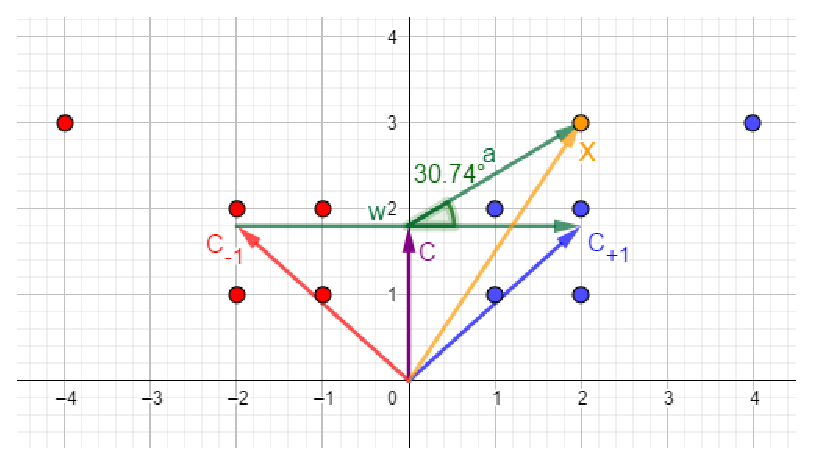
\includegraphics[width=0.5\textwidth]{kernel1} \centering \caption{Ilustração referente ao exemplo do método kernel. }
\label{kernel} 
\end{figure}

\bibliographystyle{plain}
\bibliography{referencias}

\end{document}
